\documentclass[a4paper]{article}
\usepackage{calc,amsmath,amssymb,amsfonts}
\usepackage[LGR,T1]{fontenc}
\usepackage[greek,spanish,english]{babel}
\usepackage{xcolor,longfbox,fancyhdr}
\usepackage[top=0.9165in,bottom=0.1945in,left=1.1665in,right=0.611in,noheadfoot]{geometry}
\usepackage{enumitem,hyperref}
\hypersetup{colorlinks=true,allcolors=black,pdfauthor=shin}
\usepackage[pdftex]{graphicx}
\makeatletter\newdimen\@tempdimd\makeatother
% Outline numbering
\setcounter{secnumdepth}{0}
% Text styles
\newcommand\textstyleListLabeli[1]{\foreignlanguage{spanish}{\textrm{\textbf{\textup{#1}}}}}
\newcommand\textstyleListLabelx[1]{\textrm{\textbf{#1}}}
\newcommand\textstyleListLabelxiv[1]{\textrm{\textbf{#1}}}
\newcommand\textstyleListLabelxviii[1]{\textrm{\textbf{#1}}}
\newcommand\textstyleInternetlink[1]{\textcolor{blue}{#1}}
% Pages
\fancypagestyle{Convertedi}{\fancyhf{}
  \fancyhead[L]{}
  \fancyfoot[L]{}
  \renewcommand\headrulewidth{0pt}
  \renewcommand\footrulewidth{0pt}
  \renewcommand\thepage{\arabic{page}}
}
\fancypagestyle{Standard}{\fancyhf{}
  \fancyhead[L]{}
  \fancyfoot[L]{}
  \renewcommand\headrulewidth{0pt}
  \renewcommand\footrulewidth{0pt}
  \renewcommand\thepage{\arabic{page}}
}
\fancypagestyle{Convertedvi}{\fancyhf{}
  \fancyhead[L]{}
  \fancyfoot[L]{}
  \renewcommand\headrulewidth{0pt}
  \renewcommand\footrulewidth{0pt}
  \renewcommand\thepage{\arabic{page}}
}
\fancypagestyle{Convertedv}{\fancyhf{}
  \fancyhead[L]{}
  \fancyfoot[L]{}
  \renewcommand\headrulewidth{0pt}
  \renewcommand\footrulewidth{0pt}
  \renewcommand\thepage{\arabic{page}}
}
\fancypagestyle{Convertediv}{\fancyhf{}
  \fancyhead[L]{}
  \fancyfoot[L]{}
  \renewcommand\headrulewidth{0pt}
  \renewcommand\footrulewidth{0pt}
  \renewcommand\thepage{\arabic{page}}
}
\fancypagestyle{Convertediii}{\fancyhf{}
  \fancyhead[L]{}
  \fancyfoot[L]{}
  \renewcommand\headrulewidth{0pt}
  \renewcommand\footrulewidth{0pt}
  \renewcommand\thepage{\arabic{page}}
}
\fancypagestyle{Convertedii}{\fancyhf{}
  \fancyhead[L]{}
  \fancyfoot[L]{}
  \renewcommand\headrulewidth{0pt}
  \renewcommand\footrulewidth{0pt}
  \renewcommand\thepage{\arabic{page}}
}
\pagestyle{Standard}
\author{shin}
\date{2024-06-26}
\begin{document}
\clearpage
\pagestyle{Standard}
\section{Proyecto de fundamentos de la programación}
\author{\IEEEauthorblockN{
ROTTGER EMMANUEL PARRAGUEZ LEANDRO}\\
\IEEEauthorblockA{\textit{Escuela de Ciencias de la computación} \\
\textit{UNI}\\
\texttt{rottger.parraguez.l@uni.pe}}
\and
\IEEEauthorblockN{ 
LUIS ANTONIO HEREDIA BRINGAS}\\
\IEEEauthorblockA{\textit{Escuela de Fisica} \\
\textit{UNI}\\
\texttt{luis.heredia.b@uni.pe}}
\and
\IEEEauthorblockN{ 
VALENTINO JAIR PEREZ MELO}\\
\IEEEauthorblockA{\textit{Escuela de Ingenieria Fisica.} \\
\textit{UNI}\\
\texttt{valentino.perez.m@uni.pe}}}

\maketitle
\item {\selectlanguage{spanish}
Funciones en Python}
\end{enumerate}

\bigskip

{\selectlanguage{spanish}
Las funciones en Python son bloques de código que realizan tareas específicas y pueden ser reutilizadas en diferentes
partes de un programa. Se definen con la palabra clave \textbf{def }seguida del nombre de la función y paréntesis
\textbf{()}. Pueden tener parámetros para recibir datos de entrada y pueden devolver resultados utilizando la palabra
clave \textbf{return}. Las variables definidas dentro de una función son locales, mientras que las variables definidas
fuera de una función son globales. Es una buena práctica documentar las funciones utilizando docstrings para describir
su propósito, parámetros y valores de retorno. Las funciones en Python son ciudadanos de primera clase, lo que
significa que pueden ser tratadas como cualquier otro objeto, permitiendo su uso en expresiones, asignaciones y como
argumentos de otras funciones. Además, Python admite la recursión, lo que permite a una función llamarse a sí misma, lo
que es útil para resolver problemas que pueden dividirse en casos más pequeños. En resumen, las funciones son
componentes esenciales para organizar y estructurar el código de manera modular, promoviendo la reutilización y la
claridad del código.}


\bigskip

{\selectlanguage{spanish}
Ejercicio: Crear una función que calcule el factorial de un número.}



\begin{center}
\lfbox[margin=0mm,border-style=none,padding=0mm,vertical-align=top,raise=-0.2193in]{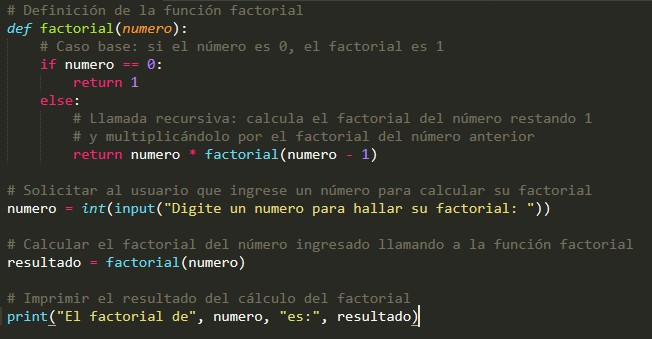
\includegraphics[width=5.5008in,height=2.8602in]{a0000-img001.jpg}}
\end{center}
{\selectlanguage{spanish}
Codigo:}

{\selectlanguage{spanish}
Ejecución:}

\begin{center}
\lfbox[margin=0mm,border-style=none,padding=0mm,vertical-align=top,raise=-0.2256in]{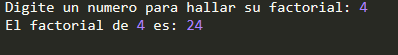
\includegraphics[width=4.1457in,height=0.5728in]{a0000-img002.png}}
\end{center}

\bigskip

\section{Cadenas en Python}

\bigskip

{\selectlanguage{spanish}
una cadena (o string) es una secuencia de caracteres. Los caracteres pueden ser letras, números, símbolos de puntuación
o incluso espacios en blanco. Las cadenas en Python se pueden definir utilizando comillas simples (') o dobles
({\textquotedbl}).}
\clearpage
\pagestyle{Convertedi}
{\selectlanguage{spanish}
Ejercicio: Escribir una función que invierta una cadena.}

\begin{center}
\lfbox[margin=0mm,border-style=none,padding=0mm,vertical-align=top,raise=-0.2563in]{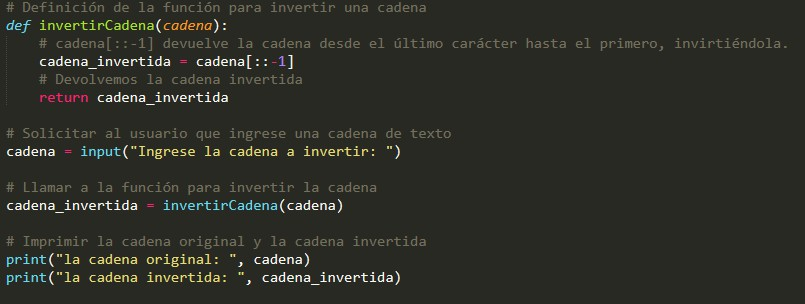
\includegraphics[width=5.8701in,height=2.2165in]{a0000-img003.jpg}}
\end{center}

\bigskip

{\selectlanguage{spanish}
Codigo:}

{\selectlanguage{spanish}
Ejecución:}

\begin{center}
\lfbox[margin=0mm,border-style=none,padding=0mm,vertical-align=top,raise=-0.2244in]{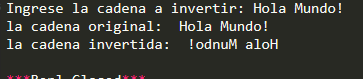
\includegraphics[width=3.7811in,height=0.8228in]{a0000-img004.png}}
\end{center}

\bigskip

\section{Referencia y asignación dinámica en Python}
{\selectlanguage{spanish}
las referencias y la asignación dinámica son conceptos fundamentales. Las referencias implican que una variable no
almacena directamente un valor, sino una referencia a un objeto en memoria, lo que permite que múltiples variables
apunten al mismo objeto. La asignación dinámica significa que las variables pueden contener diferentes tipos de valores
en diferentes momentos sin necesidad de especificar un tipo de datos. Esto proporciona flexibilidad y conveniencia
durante el desarrollo, ya que las variables pueden cambiar de tipo según sea necesario.}


\bigskip

{\selectlanguage{spanish}
\textbf{Listas: }Una lista en Python es una estructura de datos que se utiliza para almacenar una colección ordenada de
elementos. Es una de las estructuras de datos más versátiles y utilizadas en Python debido a su flexibilidad y
capacidad para manejar diferentes tipos de datos.}


\bigskip

{\selectlanguage{spanish}
Ejercicio: Crear una lista dinámica (usando listas en Python) y añadir elementos de forma interactiva.}

\clearpage
\pagestyle{Convertedii}

\lfbox[margin=0mm,border-style=none,padding=0mm,vertical-align=top]{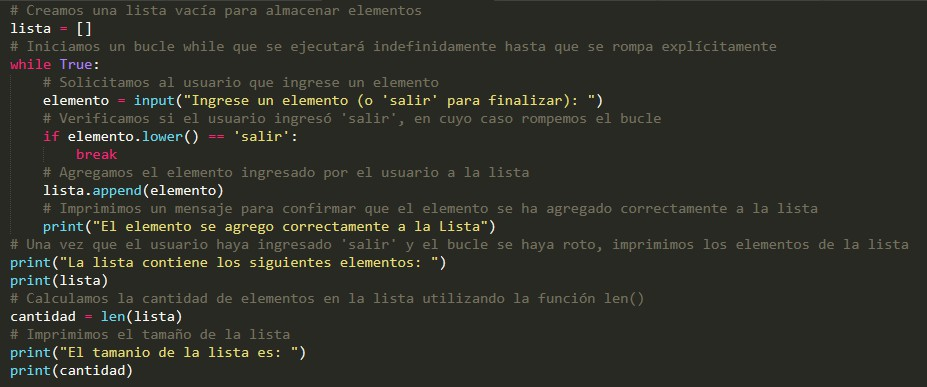
\includegraphics[width=5.8929in,height=2.4591in]{a0000-img005.jpg}}


{\selectlanguage{spanish}
Codigo:}


\bigskip

{\selectlanguage{spanish}
Ejecución:}

\begin{center}
\lfbox[margin=0mm,border-style=none,padding=0mm,vertical-align=top,raise=-0.2016in]{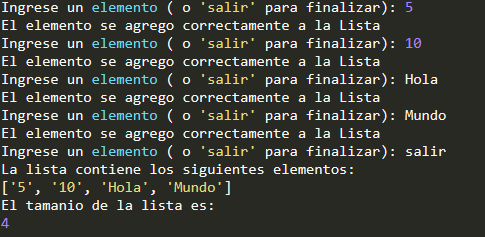
\includegraphics[width=5.0528in,height=2.4689in]{a0000-img006.png}}
\end{center}

\bigskip

\section{Diccionarios en Python}

\bigskip

{\selectlanguage{spanish}
un diccionario es una estructura de datos mutable y no ordenada que permite}

{\selectlanguage{spanish}
almacenar pares clave-valor. Las claves en un diccionario son únicas y se utilizan para acceder a los valores asociados.
Los diccionarios son heterogéneos, lo que significa que los valores pueden ser de cualquier tipo de datos, mientras que
las claves suelen ser cadenas o enteros. Los diccionarios proporcionan operaciones y métodos útiles para agregar,
eliminar y modificar elementos, así como para}

{\selectlanguage{spanish}
acceder a las claves y valores. Son ampliamente utilizados en Python debido a su flexibilidad y eficiencia para asociar
información relacionada y manipular datos de manera eficiente.}


\bigskip

{\selectlanguage{spanish}
Ejercicio: Crear una agenda telefónica utilizando diccionarios.}

\clearpage
\pagestyle{Convertediii}

\lfbox[margin=0mm,border-style=none,padding=0mm,vertical-align=top]{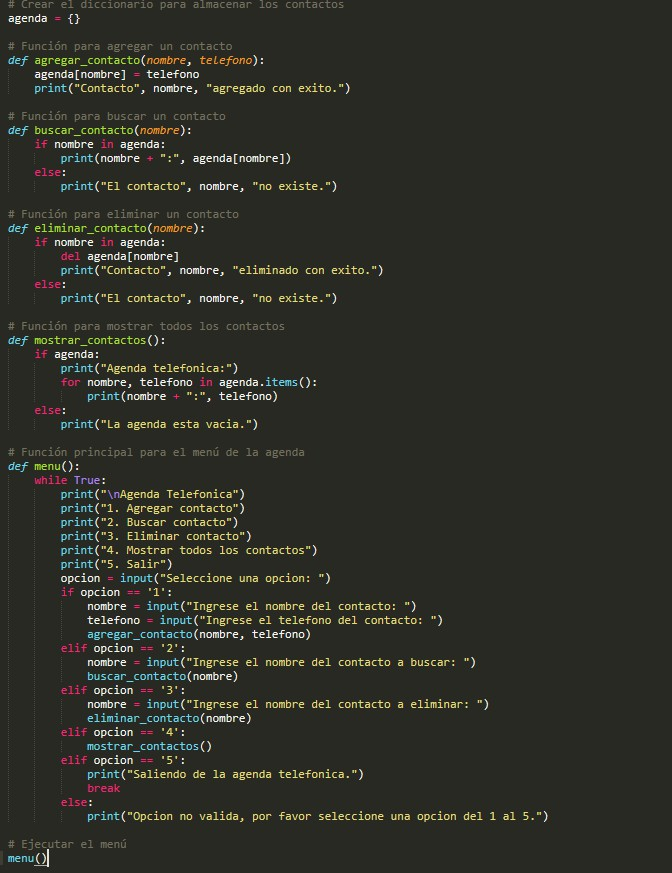
\includegraphics[width=5.8807in,height=7.639in]{a0000-img007.jpg}}


{\selectlanguage{spanish}
Codigo:}

{\selectlanguage{spanish}
Ejecución:}

\clearpage
\pagestyle{Convertediv}

\lfbox[margin=0mm,border-style=none,padding=0mm,vertical-align=top]{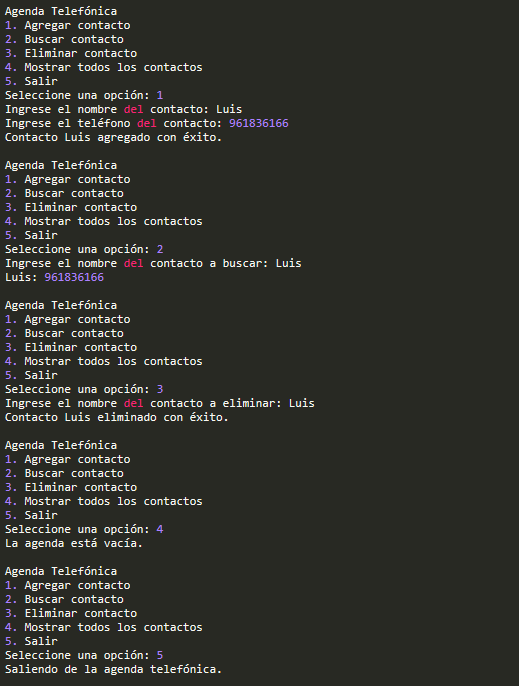
\includegraphics[width=5.4071in,height=7.1457in]{a0000-img008.png}}



\bigskip

\section{Archivos en Python}

\bigskip

{\selectlanguage{spanish}
Los archivos en Python son recursos utilizados para almacenar y recuperar datos de manera persistente en el sistema de
archivos de la computadora. Permiten conservar datos más allá de la duración de un programa en ejecución. Los archivos
pueden ser de varios tipos, como archivos de texto sin formato, archivos CSV, archivos JSON, archivos XML, archivos
binarios, entre otros. Al trabajar con archivos, se especifica un modo de apertura que indica cómo se utilizará el
archivo, como lectura, escritura o agregación. Las operaciones básicas incluyen abrir un archivo, leer o escribir datos
en él y cerrarlo cuando haya terminado. Es importante manejar los errores y excepciones que pueden ocurrir al trabajar
con archivos. En}

\clearpage
\pagestyle{Convertedv}
{\selectlanguage{spanish}
resumen, los archivos en Python son esenciales para muchas aplicaciones que requieren el almacenamiento y procesamiento
de datos de manera persistente.}

{\selectlanguage{spanish}
Ejercicio: Escribir y leer datos desde un archivo de texto.}

\begin{center}
\lfbox[margin=0mm,border-style=none,padding=0mm,vertical-align=top,raise=-0.2008in]{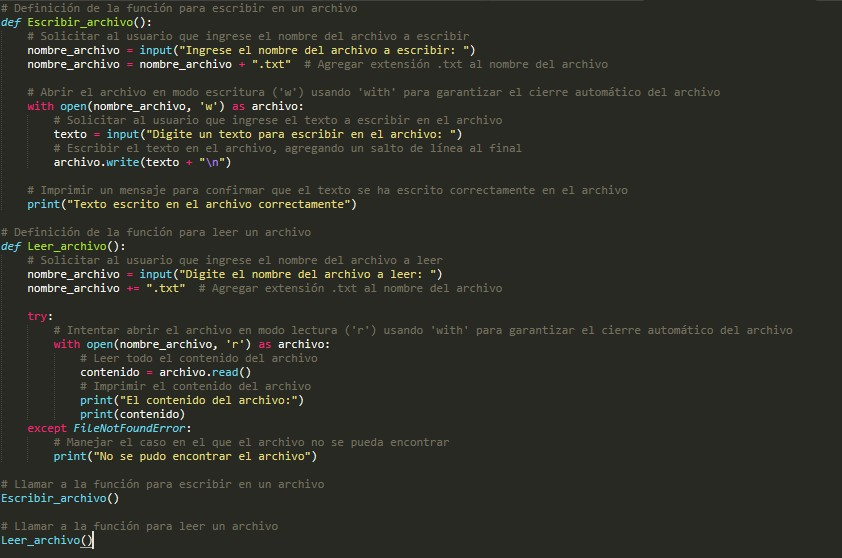
\includegraphics[width=5.8772in,height=3.8945in]{a0000-img009.jpg}}
\end{center}
{\selectlanguage{spanish}
Codigo:}

{\selectlanguage{spanish}
Ejecución:}

\begin{center}
\lfbox[margin=0mm,border-style=none,padding=0mm,vertical-align=top,raise=-0.2244in]{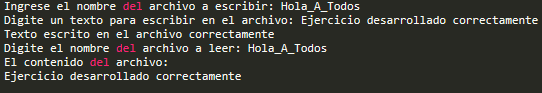
\includegraphics[width=5.6457in,height=0.9689in]{a0000-img010.png}}
\end{center}
\begin{center}
\lfbox[margin=0mm,border-style=none,padding=0mm,vertical-align=top,raise=-1.2598in]{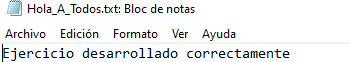
\includegraphics[width=3.6457in,height=0.6457in]{a0000-img011.png}}
\end{center}

\bigskip


\bigskip


\bigskip

\section{Clases en Python}

\bigskip

{\selectlanguage{spanish}
una clase es una plantilla que se utiliza para crear objetos. Las clases encapsulan datos y funcionalidad relacionados
en una sola entidad, lo que facilita la organización y el mantenimiento del código. Las clases pueden tener atributos
que representan datos asociados con los objetos y métodos que operan en esos datos. Además, las clases admiten la
herencia, lo que permite crear una jerarquía de clases donde las subclases pueden extender o modificar el
comportamiento de las superclases. Las clases también admiten el polimorfismo, lo que significa que diferentes objetos
pueden responder al mismo mensaje de manera diferente. En resumen, las clases en Python son una parte fundamental de la
programación orientada a objetos y proporcionan una forma eficaz de modelar entidades del mundo real y estructurar el
código de manera modular y reutilizable.}

\clearpage
\pagestyle{Convertedvi}
{\selectlanguage{spanish}
Ejercicio : Definir una clase Persona con atributos nombre y edad, y un método para mostrar estos datos.}



\begin{center}
\lfbox[margin=0mm,border-style=none,padding=0mm,vertical-align=top,raise=-0.2008in]{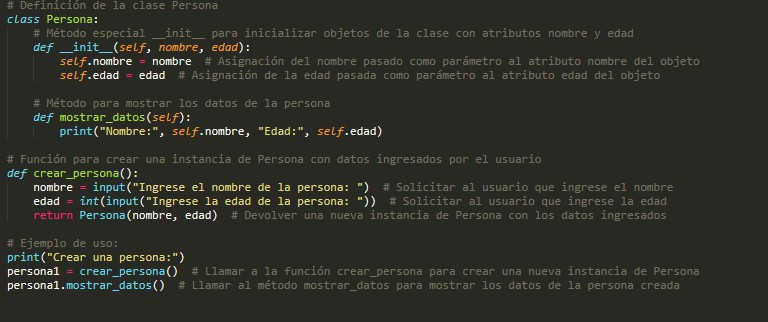
\includegraphics[width=5.922in,height=2.4819in]{a0000-img012.jpg}}
\end{center}

\bigskip

{\selectlanguage{spanish}
Codigo:}

{\selectlanguage{spanish}
Ejecución:}

\begin{center}
\lfbox[margin=0mm,border-style=none,padding=0mm,vertical-align=top,raise=-0.2189in]{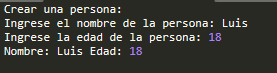
\includegraphics[width=2.8854in,height=0.7602in]{a0000-img013.png}}
\end{center}
\bigskip


\bigskip

\bigskip


\bigskip

\bigskip


\bigskip


\bigskip


\bigskip


\bigskip


\bigskip


\bigskip


\bigskip


\bigskip


\bigskip


\bigskip


\bigskip


\bigskip


\bigskip


\bigskip


\bigskip


\bigskip


\bigskip


\bigskip


\bigskip


\bigskip


\bigskip


\bigskip


\bigskip


\bigskip


\bigskip


\bigskip


\bigskip


\bigskip


\bigskip


\bigskip


\bigskip


\bigskip


\bigskip


\bigskip


\bigskip


\bigskip


\bigskip


\bigskip


\bigskip


\bigskip

{\centering\selectlanguage{spanish}
\textbf{\textit{Proyecto de Fundamentos de la programación parte 2}}
\par}


\bigskip

{\selectlanguage{spanish}
\textbf{Introducción:}}


\bigskip

{\selectlanguage{spanish}
Continuando con la segunda parte del proyecto, sean desarrollado cuatro problemas básicos que abarcan diferentes
aspectos fundamentales de la programación en python. Estos problemas son: }

\begin{itemize}[series=listWWNumii,label=\textstyleListLabelx{{}-}]
\item {\selectlanguage{spanish}
Crear una calculadora que pueda realizar operaciones básicas (suma, resta, \ multiplicación, división).}
\item {\selectlanguage{spanish}
un juego de adivinanza de números }
\item {\selectlanguage{spanish}
un conversor de monedas \ }
\item {\selectlanguage{spanish}
una aplicación de gestión de tareas}
\end{itemize}
{\selectlanguage{spanish}
El objetivo de este informe es presentar una descripción detallada de cada proyecto, su funcionalidad y el proceso de
desarrollo.}


\bigskip

{\selectlanguage{spanish}
\textbf{1. Calculadora de Operaciones Básicas:}}

{\selectlanguage{spanish}
La calculadora es un programa que permite realizar operaciones aritméticas básicas como suma, resta, multiplicación y
división. Este problema haremos uso de funciones y de la validación de entradas del usuario para el uso optimo.}


\bigskip

{\selectlanguage{spanish}
\textbf{Codigo:}}

\begin{center}
\lfbox[margin-right=0.1252in,margin-left=0.1252in,margin-top=0mm,margin-bottom=0mm,border-style=none,padding=0mm,vertical-align=top,raise=-0.3307in]{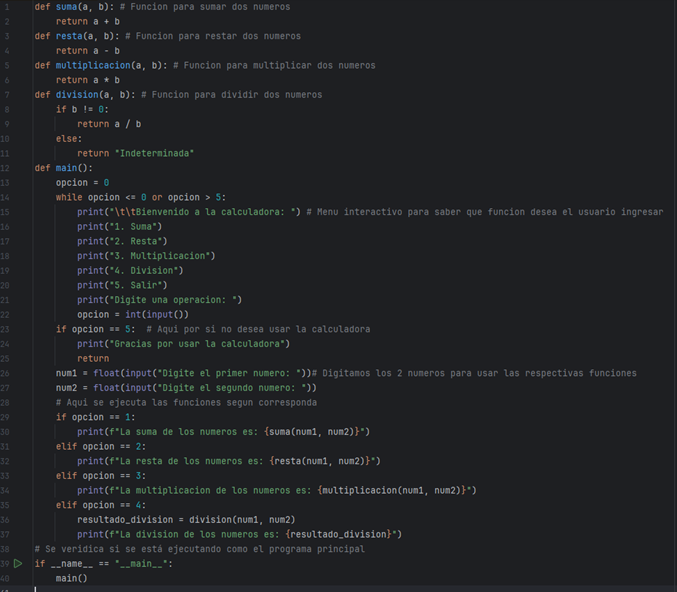
\includegraphics[width=7.052in,height=6.1681in]{a0000-img014.png}}
\end{center}

\bigskip


\bigskip


\bigskip


\bigskip


\bigskip


\bigskip


\bigskip


\bigskip


\bigskip


\bigskip


\bigskip


\bigskip


\bigskip


\bigskip


\bigskip


\bigskip


\bigskip


\bigskip


\bigskip


\bigskip


\bigskip


\bigskip


\bigskip


\bigskip


\bigskip


\bigskip


\bigskip


\bigskip


\bigskip


\bigskip


\bigskip


\bigskip


\bigskip


\bigskip


\bigskip


\bigskip


\bigskip


\bigskip

{\selectlanguage{spanish}
\textbf{Funcionalidad:}}


\bigskip

\begin{itemize}[resume*=listWWNumii]
\item {\selectlanguage{spanish}
\textbf{Operaciones:} La calculadora puede realizar las operaciones de suma, resta, multiplicación y división.}
\item {\selectlanguage{spanish}
\textbf{Validación:} El programa valida las entradas para asegurarse de que sean números y maneja errores como la
división por cero.}
\item {\selectlanguage{spanish}
\textbf{Interfaz de Usuario:} La calculadora presenta una interfaz simple donde el usuario puede introducir dos números
y seleccionar la operación deseada.}
\end{itemize}
{\selectlanguage{spanish}
\textbf{Proceso de Desarrollo:}}


\bigskip

{\selectlanguage{spanish}
Para el desarrollo de este codigo tuvimos en cuenta estos puntos clave}

\begin{itemize}[series=listWWNumiii,label=\textstyleListLabelxiv{{}-}]
\item {\selectlanguage{spanish}
Diseño de la interfaz de usuario.}
\item {\selectlanguage{spanish}
Implementación de funciones para cada operación.}
\item {\selectlanguage{spanish}
Adición de validaciones y manejo de errores}
\end{itemize}
{\selectlanguage{spanish}
\textbf{Consola:}}



\begin{center}
\lfbox[margin-right=0.1346in,margin-left=0.1252in,margin-top=0mm,margin-bottom=0mm,border-style=none,padding=0mm,vertical-align=top,raise=-0.1035in]{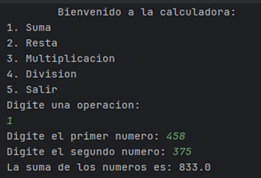
\includegraphics[width=2.7398in,height=1.8744in]{a0000-img015.png}}
\end{center}
\begin{center}
\lfbox[margin-right=0.1252in,margin-top=0mm,margin-bottom=0mm,margin-left=0mm,border-style=none,padding=0mm,vertical-align=top,raise=-0.1244in]{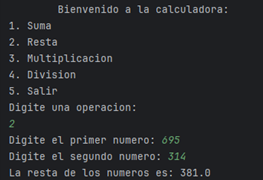
\includegraphics[width=2.7189in,height=1.8563in]{a0000-img016.png}}
\end{center}

\bigskip


\bigskip


\bigskip


\bigskip


\bigskip


\bigskip


\bigskip


\bigskip


\bigskip


\bigskip



\begin{center}
\lfbox[margin-right=0.1252in,margin-left=0.1252in,margin-top=0mm,margin-bottom=0mm,border-style=none,padding=0mm,vertical-align=top,raise=-0.15in]{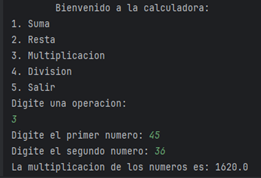
\includegraphics[width=2.7189in,height=1.8543in]{a0000-img017.png}}
\end{center}


\begin{center}
\lfbox[margin-right=0.1252in,margin-bottom=0.0091in,margin-left=0.1252in,margin-top=0mm,border-style=none,padding=0mm,vertical-align=top,raise=-0.0161in]{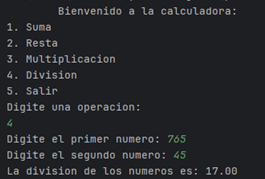
\includegraphics[width=2.7602in,height=1.8661in]{a0000-img018.png}}
\end{center}

\bigskip


\bigskip


\bigskip


\bigskip


\bigskip


\bigskip


\bigskip


\bigskip


\bigskip


\bigskip



\begin{center}
\lfbox[margin-right=0.1346in,margin-left=0.1252in,margin-top=0mm,margin-bottom=0mm,border-style=none,padding=0mm,vertical-align=top,raise=-0.011in]{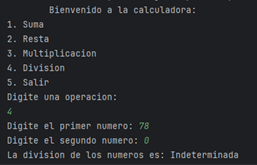
\includegraphics[width=2.802in,height=1.7291in]{a0000-img019.png}}
\end{center}
\begin{center}
\lfbox[margin-right=0.1335in,margin-left=0.1252in,margin-top=0mm,margin-bottom=0mm,border-style=none,padding=0mm,vertical-align=top,raise=-0.0102in]{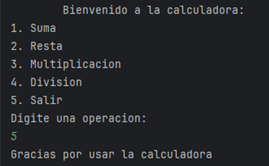
\includegraphics[width=2.6799in,height=1.7189in]{a0000-img020.png}}
\end{center}

\bigskip


\bigskip


\bigskip


\bigskip


\bigskip


\bigskip


\bigskip


\bigskip


\bigskip


\bigskip


\bigskip


\bigskip


\bigskip


\bigskip


\bigskip


\bigskip


\bigskip


\bigskip


\bigskip

{\selectlanguage{spanish}
\textbf{2. Juego de Adivinanza de Números:}}

{\selectlanguage{spanish}
Este juego consiste en que el programa elige un número aleatorio y el usuario intenta adivinarlo. El programa
proporciona pistas indicando si el número adivinado es mayor o menor que el número ha encontrar.}

{\selectlanguage{spanish}
\textbf{Observacion: }}

{\selectlanguage{spanish}
Puse el paramtro de 1 a 100 para tener un rango a encontrar}

{\selectlanguage{spanish}
\textbf{Codigo:}}


\bigskip


\bigskip



\begin{center}
\lfbox[margin-right=0.1252in,margin-left=0.1252in,margin-top=0mm,margin-bottom=0mm,border-style=none,padding=0mm,vertical-align=top,raise=-0.0764in]{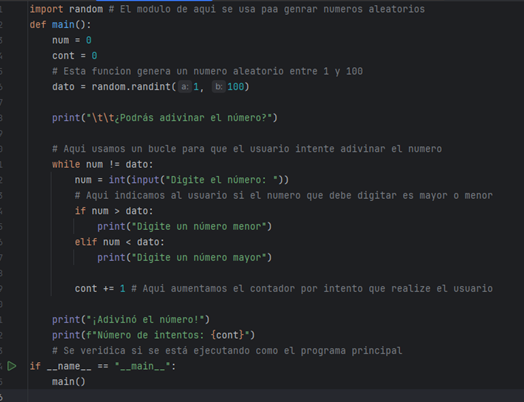
\includegraphics[width=5.4583in,height=4.1929in]{a0000-img021.png}}
\end{center}

\bigskip


\bigskip


\bigskip


\bigskip


\bigskip


\bigskip


\bigskip


\bigskip


\bigskip


\bigskip


\bigskip


\bigskip


\bigskip


\bigskip


\bigskip


\bigskip


\bigskip


\bigskip


\bigskip


\bigskip


\bigskip


\bigskip


\bigskip


\bigskip


\bigskip

{\selectlanguage{spanish}
\textbf{Funcionalidad:}}


\bigskip

\begin{itemize}[resume*=listWWNumiii]
\item {\selectlanguage{spanish}
\textbf{Generación de Números:} El programa genera un número aleatorio dentro de un rango predefinido.}
\item {\selectlanguage{spanish}
\textbf{Interacción con el Usuario:} El usuario introduce su adivinanza y el programa le indica si el número es mayor o
menor que el número objetivo.}
\item {\selectlanguage{spanish}
\textbf{Intentos:} El programa puede limitar el número de intentos o permitir intentos ilimitados.}
\end{itemize}
{\selectlanguage{spanish}
\textbf{Proceso de Desarrollo:}}


\bigskip

{\selectlanguage{spanish}
Para el desarrollo de este codigo tuvimos en cuenta estos puntos clave}

\begin{itemize}[resume*=listWWNumiii]
\item {\selectlanguage{spanish}
\textbf{Implementación de la generación de números aleatorios.}}
\item {\selectlanguage{spanish}
\textbf{Creación de la lógica para comparar el número adivinado con el número objetivo.}}
\item {\selectlanguage{spanish}
\textbf{Diseño de la interacción con el usuario.}}
\end{itemize}

\bigskip


\bigskip


\bigskip


\bigskip


\bigskip


\bigskip


\bigskip


\bigskip


\bigskip


\bigskip

{\selectlanguage{spanish}
\textbf{Consola:}}

\begin{center}
\lfbox[margin-right=0.1252in,margin-left=0.1252in,margin-top=0mm,margin-bottom=0mm,border-style=none,padding=0mm,vertical-align=top,raise=-0.3807in]{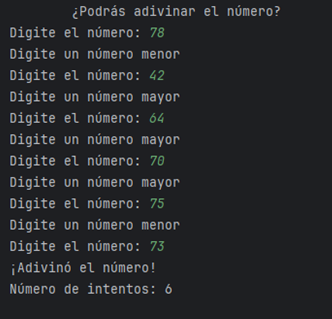
\includegraphics[width=3.4602in,height=3.3228in]{a0000-img022.png}}
\end{center}


\begin{center}
\lfbox[margin-right=0.1252in,margin-left=0.1252in,margin-top=0mm,margin-bottom=0mm,border-style=none,padding=0mm,vertical-align=top,raise=-0.0799in]{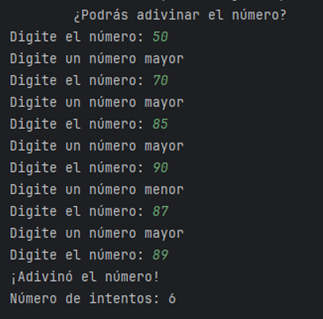
\includegraphics[width=3.3646in,height=3.3228in]{a0000-img023.png}}
\end{center}

\bigskip


\bigskip


\bigskip


\bigskip


\bigskip


\bigskip


\bigskip


\bigskip


\bigskip


\bigskip


\bigskip


\bigskip


\bigskip


\bigskip


\bigskip


\bigskip


\bigskip


\bigskip


\bigskip


\bigskip

{\selectlanguage{spanish}
\textbf{3. Conversor de Monedas:}}

{\selectlanguage{spanish}
Este programa convierte entre diferentes monedas utilizando tasas de cambio predefinidas. El usuario puede seleccionar
las monedas de origen y destino, y el programa calcula el equivalente en la moneda deseada.}

{\selectlanguage{spanish}
\textbf{Codigo:}}

\begin{center}
\lfbox[margin-right=0.1252in,margin-bottom=0.0083in,margin-top=0mm,margin-left=0mm,border-style=none,padding=0mm,vertical-align=top,raise=-0.2492in]{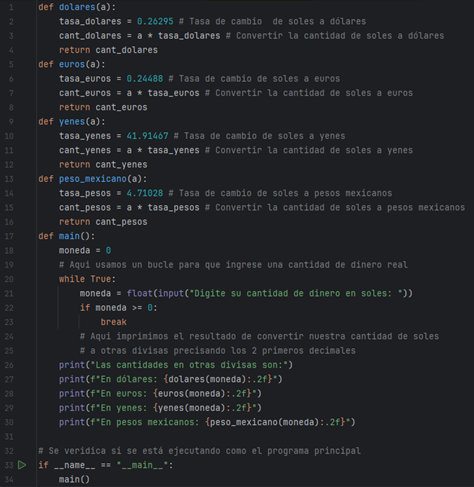
\includegraphics[width=4.9374in,height=5.0752in]{a0000-img024.png}}
\end{center}

\bigskip


\bigskip


\bigskip


\bigskip


\bigskip


\bigskip


\bigskip


\bigskip


\bigskip


\bigskip


\bigskip


\bigskip


\bigskip


\bigskip


\bigskip


\bigskip


\bigskip


\bigskip


\bigskip


\bigskip


\bigskip


\bigskip


\bigskip


\bigskip


\bigskip


\bigskip


\bigskip


\bigskip


\bigskip


\bigskip


\bigskip


\bigskip


\bigskip

{\selectlanguage{spanish}
\textbf{Funcionalidad:}}

\begin{itemize}[series=listWWNumiv,label=\textstyleListLabelxviii{{}-}]
\item {\selectlanguage{spanish}
Selección de Monedas: El usuario puede seleccionar la moneda de origen y la moneda de destino.}
\item {\selectlanguage{spanish}
Tasas de Cambio: El programa utiliza tasas de cambio predefinidas para realizar la conversión en este caso usamos 4.}
\item {\selectlanguage{spanish}
Cálculo: El programa calcula el valor convertido basado en la tasa de cambio seleccionada.}
\end{itemize}
{\selectlanguage{spanish}
\textbf{Proceso de Desarrollo:}}

{\selectlanguage{spanish}
El desarrollo del conversor de monedas incluyó:}

\begin{itemize}[resume*=listWWNumiv]
\item {\selectlanguage{spanish}
\textbf{Definición de las tasas de cambio.}}
\item {\selectlanguage{spanish}
\textbf{Implementación de la lógica para realizar la conversión.}}
\item {\selectlanguage{spanish}
\textbf{Creación de la interfaz de usuario para seleccionar las monedas y mostrar el resultado.}}
\end{itemize}
{\selectlanguage{spanish}
\textbf{Consola:}}

\begin{center}
\lfbox[margin-right=0.1252in,margin-bottom=0.0075in,margin-left=0.1252in,margin-top=0mm,border-style=none,padding=0mm,vertical-align=top,raise=-0.2874in]{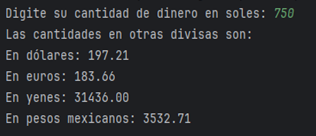
\includegraphics[width=3.5835in,height=1.4299in]{a0000-img025.png}}
\end{center}
\begin{center}
\lfbox[margin-right=0.1272in,margin-left=0.1252in,margin-top=0mm,margin-bottom=0mm,border-style=none,padding=0mm,vertical-align=top,raise=-0.298in]{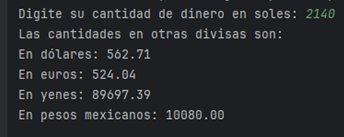
\includegraphics[width=3.2902in,height=1.4165in]{a0000-img026.png}}
\end{center}

\bigskip


\bigskip


\bigskip


\bigskip


\bigskip


\bigskip


\bigskip


\bigskip


\bigskip


\bigskip

{\selectlanguage{spanish}
\textbf{4. Aplicación de Gestión de Tareas:}}

{\selectlanguage{spanish}
Esta aplicación permite a los usuarios agregar, eliminar y marcar tareas como completadas. Es una herramienta útil para
la gestión personal de tareas y pendientes.}

{\selectlanguage{spanish}
\textbf{Codigo:}}

\begin{center}
\lfbox[margin-right=0.1252in,margin-left=0.1252in,margin-top=0mm,margin-bottom=0mm,border-style=none,padding=0mm,vertical-align=top,raise=-0.298in]{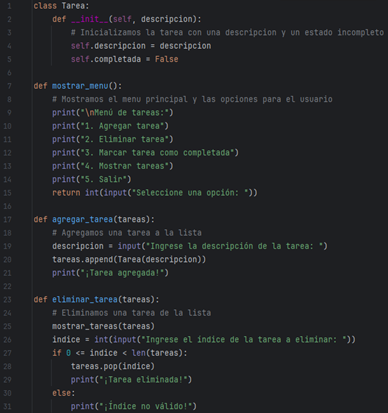
\includegraphics[width=4.0417in,height=4.3016in]{a0000-img027.png}}
\end{center}


\begin{center}
\lfbox[margin-right=0.1252in,margin-left=0.1252in,margin-top=0mm,margin-bottom=0mm,border-style=none,padding=0mm,vertical-align=top,raise=-0.1327in]{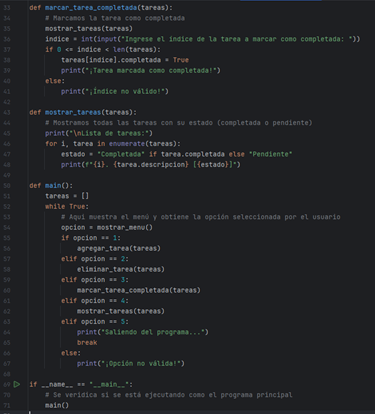
\includegraphics[width=3.9055in,height=4.3161in]{a0000-img028.png}}
\end{center}

\bigskip


\bigskip


\bigskip


\bigskip


\bigskip


\bigskip


\bigskip


\bigskip


\bigskip


\bigskip


\bigskip


\bigskip


\bigskip


\bigskip


\bigskip


\bigskip


\bigskip


\bigskip


\bigskip


\bigskip


\bigskip


\bigskip


\bigskip


\bigskip


\bigskip


\bigskip


\bigskip


\bigskip


\bigskip


\bigskip


\bigskip

{\selectlanguage{spanish}
\textbf{Funcionalidad:}}

\begin{itemize}[resume*=listWWNumiv]
\item {\selectlanguage{spanish}
\textbf{Agregar Tareas:} \ Los usuarios pueden agregar nuevas tareas a la lista.}
\item {\selectlanguage{spanish}
\textbf{Eliminar Tareas:} Los usuarios pueden eliminar tareas de la lista.}
\item {\selectlanguage{spanish}
\textbf{Marcar como Completadas:} Los usuarios pueden marcar tareas como completadas.}
\end{itemize}
{\selectlanguage{spanish}
\textbf{Proceso de Desarrollo:}}

{\selectlanguage{spanish}
El desarrollo de la aplicación de gestión de tareas incluyó:}

\begin{itemize}[resume*=listWWNumiv]
\item {\selectlanguage{spanish}
\textbf{Implementación de la funcionalidad para agregar, eliminar y marcar tareas.}}
\item {\selectlanguage{spanish}
\textbf{Diseño de la interfaz de usuario para mostrar y gestionar las tareas.}}
\item {\selectlanguage{spanish}
\textbf{Manejo del almacenamiento de tareas, ya sea en memoria o en un archivo.}}
\end{itemize}
{\selectlanguage{spanish}
\textbf{Consola:}}

\begin{center}
\lfbox[margin-right=0.1252in,margin-left=0.1252in,margin-top=0mm,margin-bottom=0mm,border-style=none,padding=0mm,vertical-align=top,raise=-0.3063in]{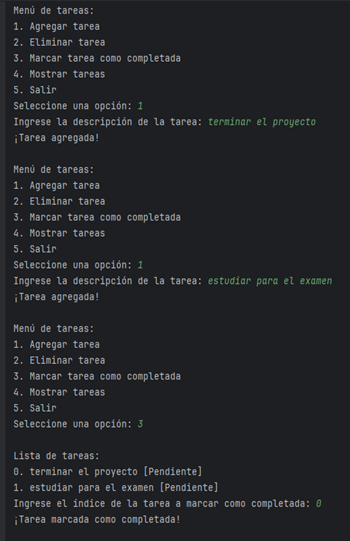
\includegraphics[width=3.6457in,height=5.6354in]{a0000-img029.png}}
\end{center}


\begin{center}
\lfbox[margin-right=0.1252in,margin-left=0.1252in,margin-top=0mm,margin-bottom=0mm,border-style=none,padding=0mm,vertical-align=top,raise=-0.0055in]{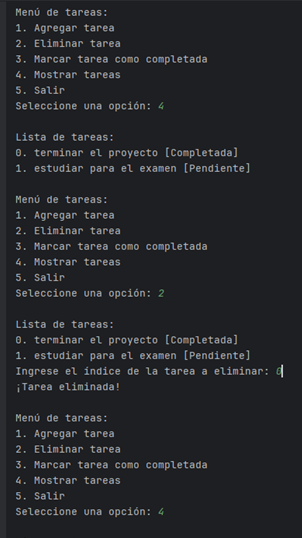
\includegraphics[width=3.1457in,height=5.6043in]{a0000-img030.png}}
\end{center}

\bigskip


\bigskip


\bigskip


\bigskip


\bigskip


\bigskip


\bigskip


\bigskip


\bigskip


\bigskip


\bigskip


\bigskip


\bigskip


\bigskip


\bigskip


\bigskip


\bigskip



\begin{center}
\lfbox[margin-right=0.1252in,margin-left=0.1252in,margin-top=0mm,margin-bottom=0mm,border-style=none,padding=0mm,vertical-align=top,raise=-0.1453in]{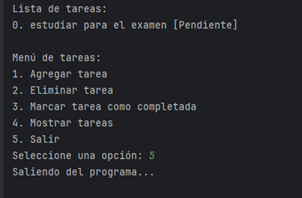
\includegraphics[width=3.1457in,height=2.0665in]{a0000-img031.png}}
\end{center}

\bigskip


\bigskip


\bigskip


\bigskip


\bigskip


\bigskip


\bigskip


\bigskip


\bigskip


\bigskip


\bigskip


\bigskip


\bigskip


\bigskip


\bigskip


\bigskip


\bigskip


\bigskip


\bigskip


\bigskip


\bigskip


\bigskip


\bigskip


\bigskip


\bigskip


\bigskip


\bigskip


\bigskip


\bigskip

{\selectlanguage{spanish}
\textbf{\textcolor{black}{Desarrollo Web con Flask/Django: Crear una aplicación web simple utilizando Flask o Django}}}


\bigskip

{\selectlanguage{spanish}
\textcolor{black}{Flask es un }\textbf{\textcolor{black}{framework}}\textcolor{black}{ (un esquema o marco de trabajo
que ofrece una estructura base para elaborar un proyecto con objetivos específicos, una especie de plantilla que sirve
como punto de partida para la organización y desarrollo de software) }\textbf{\textcolor{black}{ligero y
flexible}}\textcolor{black}{ para el desarrollo de aplicaciones web en Python. Permite crear aplicaciones web
rápidamente y con una }\textbf{\textcolor{black}{sintaxis sencilla}}\textcolor{black}{, proporcionando herramientas
para el manejo de peticiones HTTP, manejo de sesiones, autenticación de usuarios, entre otros. Flask es ideal para
crear aplicaciones web simples y rápidas, pero también es lo suficientemente potente y extensible para desarrollar
aplicaciones web más complejas. Es una herramienta muy popular en la comunidad de desarrollo web en Python.}}

{\selectlanguage{spanish}
\textcolor{black}{Para alguien experimentado, cuando piensa en Python, el framework de facto que llega a su mente es el
framework }\href{https://www.djangoproject.com/}{\textstyleInternetlink{\textcolor{black}{Django}}}\textcolor{black}{.
Pero desde una perspectiva de principiantes (en este caso nosotros) de Python, Flask es más fácil para comenzar que en
comparación con Django.}}


\bigskip

{\selectlanguage{spanish}
\textbf{\textcolor{black}{PASOS:}}}

{\selectlanguage{spanish}
\textcolor{black}{Primero debemos }\textbf{\textcolor{black}{instalar Python}}\textcolor{black}{, de preferencia
versiones }\textbf{\textcolor{black}{+3.7}}\textcolor{black}{; luego usando el comando
}\textbf{\textcolor{black}{pip}}\textcolor{black}{ en el terminal procedemos a }\textbf{\textcolor{black}{instalar el
Flask}}\textcolor{black}{:}}


\lfbox[margin=0mm,border-style=none,padding=0mm,vertical-align=top]{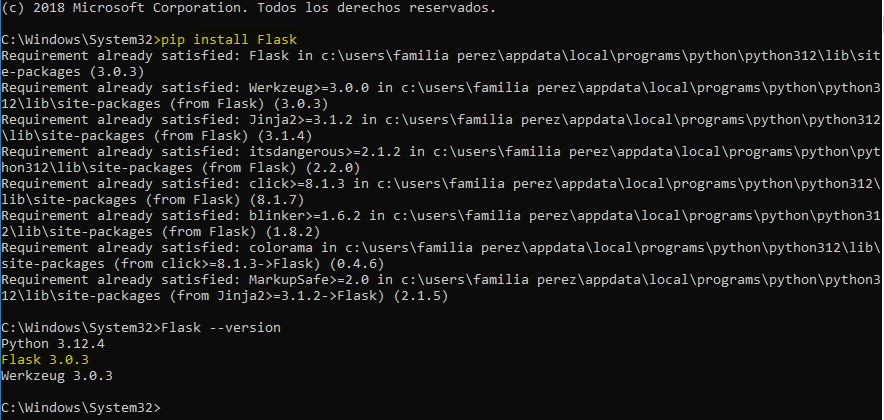
\includegraphics[width=6.3665in,height=3.2811in]{a0000-img032.png}}


{\selectlanguage{spanish}
\textcolor{black}{Procedemos a crea un archivo de Python en nuestro editor de texto favorito (en este caso elegimos
}\textbf{\textcolor{black}{VS Code}}\textcolor{black}{) y lo nombramos
}\textit{\textcolor{black}{app1.py}}\textcolor{black}{. En este archivo, comenzamos importando Flask y creando una
instancia de la aplicación:}}


\lfbox[margin=0mm,border-style=none,padding=0mm,vertical-align=top]{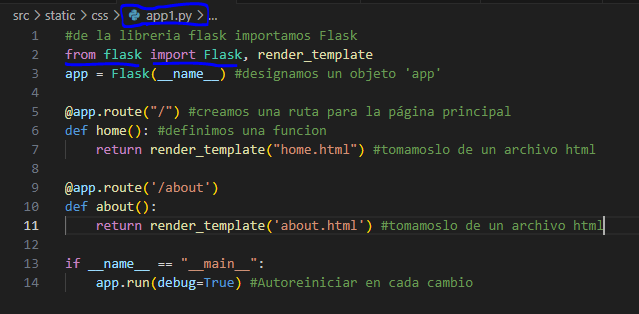
\includegraphics[width=6.1374in,height=3.0161in]{a0000-img033.png}}



\bigskip

{\selectlanguage{spanish}
\textcolor{black}{Guardamos el archivo y lo ejecutamos en la terminal utilizando el comando
}\textbf{\textcolor{black}{python app1.py}}\textcolor{black}{. Flask iniciará un servidor local y podremos acceder a la
aplicación web en nuestro navegador ingresando la URL }\url{http://localhost:5000/}\textcolor{black}{. (utilizamos
Chrome)}}


\lfbox[margin=0mm,border-style=none,padding=0mm,vertical-align=top]{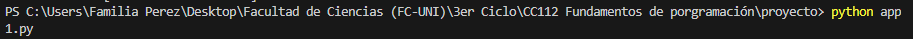
\includegraphics[width=6.1374in,height=0.2626in]{a0000-img034.png}}



\bigskip

{\selectlanguage{spanish}
\textcolor{black}{Nosotros en realidad no queremos estar enviando tan solo texto, queremos enviar
HTML$\text{\textgreek{’}}$s, ya que cuando creamos un sitio web tenemos que crear páginas web con interfaces y así
saber sobre qué trata este sitio web.}}

{\selectlanguage{spanish}
\textcolor{black}{En este caso creamos una carpeta llamada $\text{\textgreek{‘}}$templates$\text{\textgreek{’}}$ que
contenga archivos HTML's y en cada ruta retornaremos un archivo HTML, pero para ello primero importamos desde Flask
$\text{\textgreek{‘}}$render\_template$\text{\textgreek{’}}$}}


\lfbox[margin=0mm,border-style=none,padding=0mm,vertical-align=top]{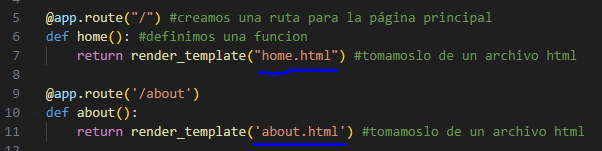
\includegraphics[width=6.1374in,height=1.6252in]{a0000-img035.png}}


\centering
\lfbox[margin=0mm,border-style=none,padding=0mm,vertical-align=top]{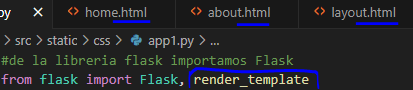
\includegraphics[width=5.6146in,height=1.2236in]{a0000-img036.png}}
\par

\bigskip

{\selectlanguage{spanish}
\textcolor{black}{Utilizamos una plantilla }\textbf{\textcolor{black}{HTML:5}}\textcolor{black}{ que viene por default
en VS Code y nos facilita bastante, usamos esto en primera instancia en }\textbf{\textcolor{black}{home.html}}}


\bigskip

{\selectlanguage{spanish}
\textcolor{black}{Como nuestro programa estará en un proceso de prueba, y lo estamos modificando y probando cada
instante, para no estar borrando y volviendo a ejecutar, queremos que se auto reinicie en cada cambio}}


\lfbox[margin=0mm,border-style=none,padding=0mm,vertical-align=top]{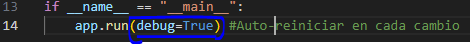
\includegraphics[width=5.6752in,height=0.5311in]{a0000-img037.png}}



\bigskip


\bigskip

{\selectlanguage{spanish}
\textcolor{black}{Para estilizar mejor nuestra página creamos una carpeta
$\text{\textgreek{‘}}$}\textbf{\textcolor{black}{static$\text{\textgreek{’}}$}}\textcolor{black}{, dentro una carpeta
$\text{\textgreek{‘}}$}\textbf{\textcolor{black}{css$\text{\textgreek{’}}$}}\textcolor{black}{ y dentro un archivo
$\text{\textgreek{‘}}$}\textbf{\textcolor{black}{main.css$\text{\textgreek{’}}$}}\textcolor{black}{; luego enlazamos el
archivo css con el HTML.}}


\bigskip

{\selectlanguage{spanish}
\textcolor{black}{Para mejorar nuestro diseño haremos uso de algún freamwork de css, en este caso usaremos
}\textbf{\textcolor{black}{Bootstrap}}\textcolor{black}{ que es bien conocido; es un freamwork que nos proporciona
estilos de css ya creados debido al poco conocimiento de css que tenemos, además que nos ahorra tiempo en lugar de
escribir código css puro.}}


\bigskip

{\selectlanguage{spanish}
\textcolor{black}{Copiamos en el HTML el }\textbf{\textcolor{black}{CDN}}\textcolor{black}{ para el css que aparece en
la página de Bootstrap, que no es más que una dirección de internet, en el
}\textbf{\textcolor{black}{home.html}}\textcolor{black}{.}}


\lfbox[margin=0mm,border-style=none,padding=0mm,vertical-align=top]{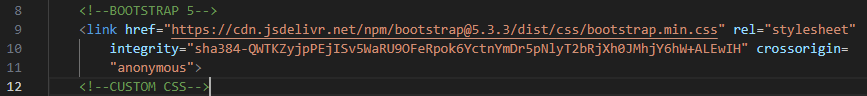
\includegraphics[width=6.1374in,height=0.6799in]{a0000-img038.png}}



\bigskip

{\selectlanguage{spanish}
\textcolor{black}{Dentro de la página de Bootstrap, en la pestaña de
}\textbf{\textcolor{black}{Navbar}}\textcolor{black}{ copiamos el código de estilo de navegación más preparada, que
contenga un }\textbf{\textcolor{black}{título y pestañas}}\textcolor{black}{ que nos conduzca a cada ruta. Modificamos
el título y el nombre de 2 pestañas que en este caso serán las únicas que usaremos.}}


\lfbox[margin=0mm,border-style=none,padding=0mm,vertical-align=top]{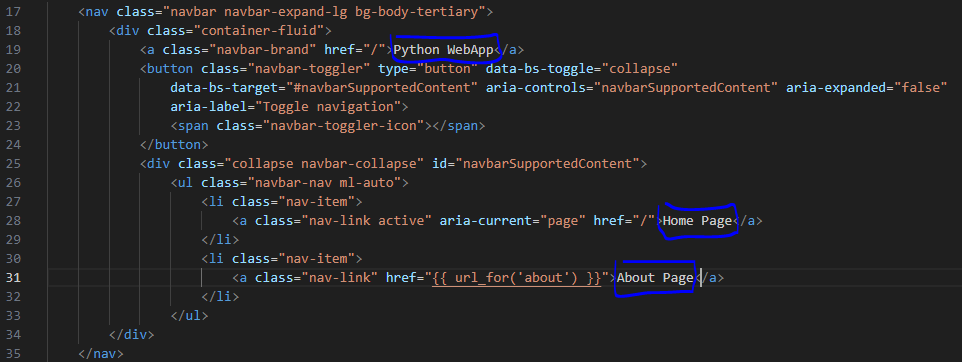
\includegraphics[width=6.1374in,height=2.552in]{a0000-img039.png}}



\bigskip

{\selectlanguage{spanish}
\textcolor{black}{Creamos ahora un tercer archivo HTML, llamado }\textbf{\textcolor{black}{layout}}\textcolor{black}{,
que nos servirá para colocar todo el código que podamos }\textit{\textcolor{black}{reutilizar}}\textcolor{black}{ que
se encontraba en }\textbf{\textcolor{black}{home.html}}\textcolor{black}{; en este caso reutilizaremos lo que se
encontraba en el head que siempre se repite, y la parte de la navegación, debajo de esta última será lo que va a
cambiar. Colocaremos un }\textbf{\textcolor{black}{$\text{\textgreek{‘}}$block
content$\text{\textgreek{’}}$}}\textcolor{black}{ y
}\textbf{\textcolor{black}{$\text{\textgreek{‘}}$endblock$\text{\textgreek{’}}$,}}\textcolor{black}{ lo que significa
que justo en estas 2 líneas de código vamos a poder colocar todo el código de otras páginas capaces de reutilizar el
contenido del }\textbf{\textcolor{black}{$\text{\textgreek{‘}}$head$\text{\textgreek{’}}$ }}\textcolor{black}{y la
}\textbf{\textcolor{black}{navegación}}}


\lfbox[margin-right=0.0102in,margin-top=0mm,margin-bottom=0mm,margin-left=0mm,border-style=none,padding=0mm,vertical-align=top]{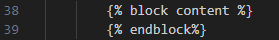
\includegraphics[width=2.9063in,height=0.4165in]{a0000-img040.png}}



\bigskip


\bigskip

\clearpage{\selectlanguage{spanish}
\textcolor{black}{Todo el código de }\textbf{\textcolor{black}{home.html}}\textcolor{black}{ y
}\textbf{\textcolor{black}{about.html}}\textcolor{black}{ va a }\textit{\textcolor{black}{extender}}\textcolor{black}{
de un archivo llamado layout.html, en los que únicamente escribimos lo que no va a repetirse, ya que el código
equivalente a ambos está en el layout; el código va }\textit{\textcolor{black}{entre $\text{\textgreek{‘}}$block
content$\text{\textgreek{’}}$ y $\text{\textgreek{‘}}$endblock$\text{\textgreek{’}}$}}\textcolor{black}{,
}\textit{\textcolor{black}{reutilizando}}\textcolor{black}{ así una porción de código en diversos archivos, navegando
fácilmente en la página.}}


\lfbox[margin=0mm,border-style=none,padding=0mm,vertical-align=top]{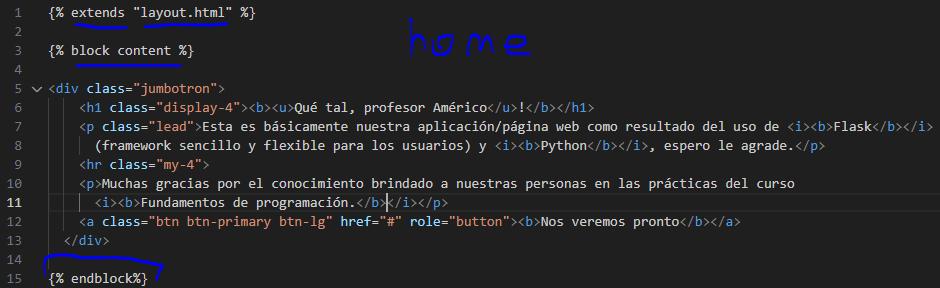
\includegraphics[width=6.1374in,height=1.8807in]{a0000-img041.png}}



\lfbox[margin=0mm,border-style=none,padding=0mm,vertical-align=top]{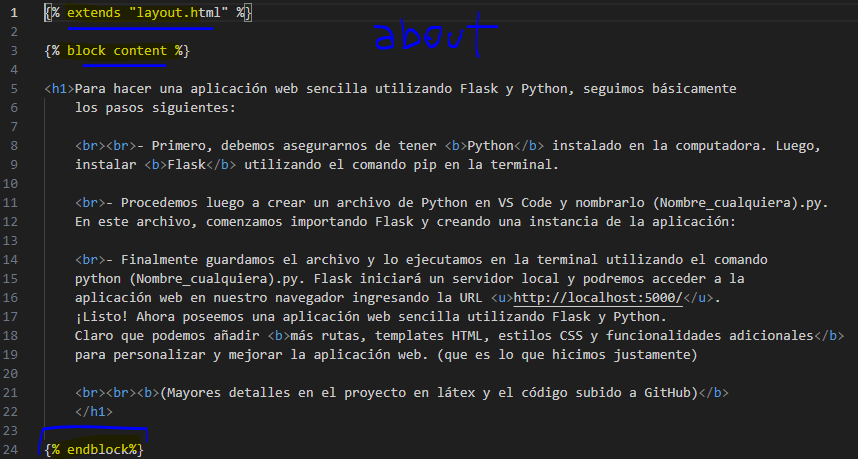
\includegraphics[width=6.1374in,height=3.2835in]{a0000-img042.png}}



\bigskip

{\selectlanguage{spanish}
\textcolor{black}{En la página de }\textbf{\textcolor{black}{Bootstrap}}\textcolor{black}{, ventana de
}\textbf{\textcolor{black}{Jumbotrom}}\textcolor{black}{, copiamos la plantilla de código en el
}\textbf{\textcolor{black}{home.html}}\textcolor{black}{ que nos proporciona un buen diseño de nuestra página principal
(de bienvenida), y lo colocamos en un }\textit{\textcolor{black}{container }}\textcolor{black}{en el
}\textbf{\textcolor{black}{layout}}\textcolor{black}{ para que esté centrado.}}


\lfbox[margin=0mm,border-style=none,padding=0mm,vertical-align=top]{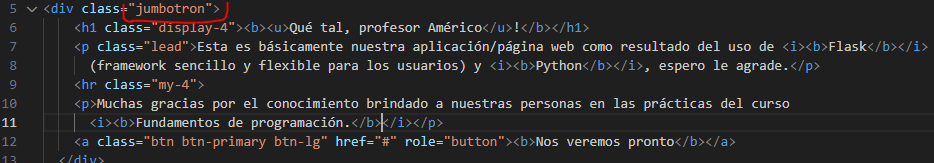
\includegraphics[width=6.1374in,height=1.0709in]{a0000-img043.png}}



\bigskip


\lfbox[margin-bottom=0.0102in,margin-top=0mm,margin-right=0mm,margin-left=0mm,border-style=none,padding=0mm,vertical-align=top]{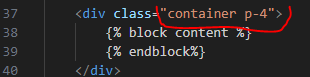
\includegraphics[width=3.2291in,height=0.802in]{a0000-img044.png}}



\bigskip

{\selectlanguage{spanish}
\textcolor{black}{Finalmente le aplicaremos un color de fondo a nuestra aplicación, para ello ingresamos a una página
del navegador llamada }\textbf{\textcolor{black}{uigradients}}\textcolor{black}{ que nos
}\textit{\textcolor{black}{proporciona degradados en código css}}\textcolor{black}{, elegimos el color que más nos
guste, copiamos su código y lo pegamos en el }\textbf{\textcolor{black}{main.css}}\textcolor{black}{.}}


\lfbox[margin=0mm,border-style=none,padding=0mm,vertical-align=top]{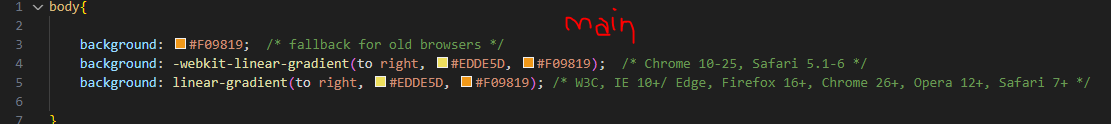
\includegraphics[width=6.1374in,height=0.6846in]{a0000-img045.png}}



\bigskip


\bigskip


\bigskip

{\selectlanguage{spanish}
\textcolor{black}{Luego de todos estos pasos, estaría completada nuestra aplicación web sencilla; cabe mencionar que
posteriormente usando }\textbf{\textcolor{black}{Flask}}\textcolor{black}{ y
}\textbf{\textcolor{black}{mysqldb}}\textcolor{black}{ podemos hacer
}\textit{\textcolor{black}{formularios}}\textcolor{black}{, }\textit{\textcolor{black}{tomar}}\textcolor{black}{
}\textit{\textcolor{black}{datos}}\textcolor{black}{ y demás. ¡Es un mundo muy grande por incursionar!}}

{\selectlanguage{spanish}
\textit{\textcolor{black}{Agradecemos a los canales:
}}\textbf{\textit{\textcolor{black}{Reolcode}}}\textit{\textcolor{black}{,
}}\textbf{\textit{\textcolor{black}{Fazt}}}\textit{\textcolor{black}{,
}}\textbf{\textit{\textcolor{black}{Condenautas}}}\textit{\textcolor{black}{,
}}\textbf{\textit{\textcolor{black}{Dari}}}\textit{\textcolor{black}{
}}\textbf{\textit{\textcolor{black}{Developer}}}\textit{\textcolor{black}{,
}}\textbf{\textit{\textcolor{black}{ikerdev}}}\textit{\textcolor{black}{ \newline
}}\textbf{\textit{\textcolor{black}{UskoKruM2010}}}\textit{\textcolor{black}{,
}}\textbf{\textit{\textcolor{black}{tavodev}}}\textit{\textcolor{black}{ y }}\textbf{\textit{\textcolor{black}{Frank
Andrade}}}\textit{\textcolor{black}{, por la información brindada en este campo en el que no estábamos completamente
familiarizados.}}}


\bigskip
\end{document}

